I decided to put this section after the Theoretical Description part since in order to better describe these related works the reader must have a good comprehension of all the basis on these models otherwise it would be completely lost. \\ 
Language models consist of systems that output the probability of a word given the context. Many times it is considered useful not only the word that can be generated but also the context itself. It, in fact, groups together very useful information that can be used for numerous activities within the world of Natural Language Processing. \\
How likely is it that a certain sequence of words will appear several times within a dataset or during inference? Unfortunately this event is very unlikely and for this reason models based simply on the frequency of appearance of these words within the dataset cannot obtain significant results.
I think this chapter can be divided in three subsection: 
\subsection{From Beginning To Recurrent Neural Network Based Models}

There are lot of related works and I think it would be interesting to start from the fist works that were using normal RNN to train models to predict next word \cite{Bengio2003} \cite{Mikolov2010}  \\
These models suffer of \textit{exposure bias}: this problem was presented by Bengio\cite{BengioSS} in 2015. This consists in the problem that training and inference are substantially different if in the training procedure you use the true token as input to generate just the next one, while in the inference you use the previously generated token to infer the next one and all the following ones. This is a big difference because in training is like you’re starting always from zero instead in the inference there is an error that increases over time due to the usage of predicted words and not real ones (that trivially you don’t have). Scheduled Sampling is a technique to solve it that uses a random variable in the train that states if to use a generated token or the true one, in order to make train and inference similar. Although it often increases performances, it was proved to be inconsistent by Huszar in 2015.\cite{Huszar} Also Professor Forcing \cite{LambTF} technique was proposed to solve this problem.

\subsubsection[TopicRNN]{TopicRNN \cite{Dieng}}
\label{sect:TopicRNN}
\textit{Anche questo modello verrà analizzato nel dettaglio visto che è rilevante all'interno del nostro modello}

\subsection{GAN Based}
The adversarial training has been used in a comprehensive manner in numerous research and applications of Computer Vision. Also in the field of Natural Language Processing many of these techniques have been developed in recent years. \\
Two of the main solutions are presented in detail below:
\subsubsection[SeqGAN]{SeqGAN \cite{Yu2016}}
\label{sect:SeqGAN}
This is an important paper inside the context of text generation using adversarial training because it introduces efficiently the usage of REINFORCE algorithm inside the generation process. \\
\textit{It will be analyzed more in detail.}

\subsubsection[RelGAN]{RelGAN \cite{RelGAN}}
\label{sect:RelGAN}
Relational Generative Adversarial Networks for Text Generation: this paper, published at the conference ICLR 2019, introduces many novelties inside this research field and achieved state of the art results. These novelties can be summerized in three points:
\begin{enumerate}
	\item \textit{Relational Memory Based Generator}: differently for many other models RelGAN does not use the typical RNN-based generator but authors has decided to use a Relational Memory \cite{Santoro}. The basic idea is to consider a steady set of memory slots and interact with these slots with a self-attention mechanism \cite{Vaswani}. The latter [Fig \ref{img:RelationalMemory}] has achieved remarkably results in many application for its ability to learn which is the best part of the memory to take information from for the following tasks.
	
	\begin{figure}[h!]
		\centering
		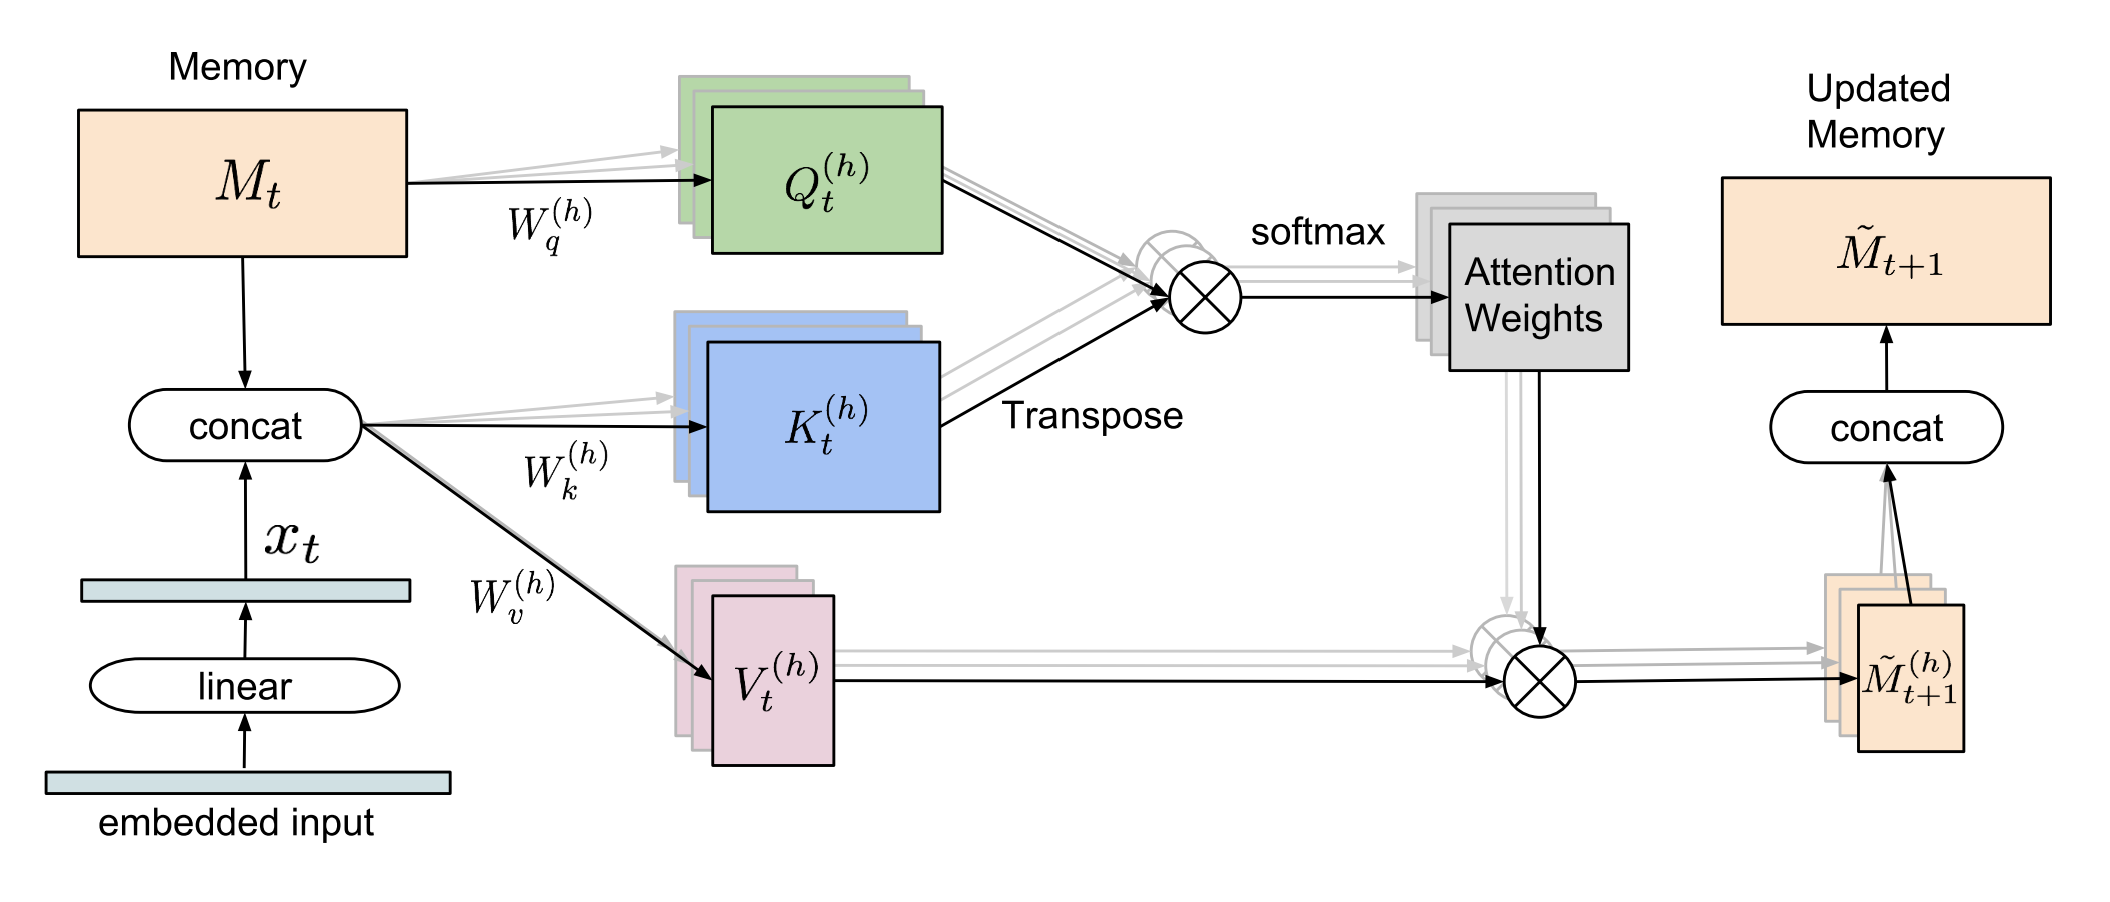
\includegraphics[width=0.8\linewidth]{Images/RelationalMemorySelfAttention.png}
		\caption{Relational Memory with Self-Attention Model}
		\label{img:RelationalMemory}
	\end{figure}
	
	\textit{Qua secondo me bisogna andare più nel dettaglio di cosa si fa effetivamente dentro una Relational Memory con anche formule etc perchè servono dopo per spiegare l'output del modello.}
	
	\item \textit{Gumbel-Softmax Relaxation}: This is the method that RelGAN uses to sample from the output distribution of the generator. As stated before in this discrete data environment it is important to have a one-hot like vector as output and many techniques were invented to deal with this problem. This is a technique used to sample from a distribution. The problem is that sampling from a multinomial distribution can be done using \myeqref{eq:ArgmaxSampling}.
	
	\begin{equation} \label{eq:ArgmaxSampling}
	y_{t} = one\_hot(arg max(o_{t})) 
	\end{equation}
	
	However, it is not possible to pass the gradient through the operation of argmax because it is not drivable. For this reason some techniques, such as Gumbel-softmax relaxation, have been invented.
	\begin{equation}
	\begin{split}
	\label{eq:gumbel}
	y_{t} = \sigma(\beta(o_{t} + g_{t})) \\
	g_{t} = -log(-log \; U_{t}) \\
	U_{t} \sim Uniform(0,1)
	\end{split}
	\end{equation}
	where $\sigma(\cdot)$ is a softmax function which is done element-wisely on its argument. \\
	It should also be consider the parameter $\beta$ that is called \textit{temperature} and it can control sample diversity and quality. Larger $\beta$ encourages more exploration to improve the diversity of the output instead smaller values of $\beta$ push to more exploitation, increasing the quality, therefore the Bleu score, conceding something on diversity. 
	\item \textit{Multiple Representation in Discriminator}: A common used discriminator in such cases is a CNN-based classifier for its ability, thanks to filters of different sizes, of collecting information from different relations between elements in the input. In this case the input is a series of one-hot vector $[r_{1} : ... : r_{T}]$ and, as proposed in previous chapter, it is important to have an embedding matrix to capture different concepts around the input sequence. It often happens that the embedding matrix is learnt through gradient propagation by the system in order to have the best possible embedded representation. In this work they propose not have one such structure but many of them in parallel, as show in [Fig \ref{img:MultipleDiscriminator}], in order to allow the network to learn different representation of the words in input. Thanks to the ablation study done at the end of the paper it is clear how this procedure is effective to push the generation forward keeping important information on the context and on the syntax situation of the sentence ($e.g.$ if a comma or a preposition is needed)
		
	\begin{figure}[h!]
		\centering
		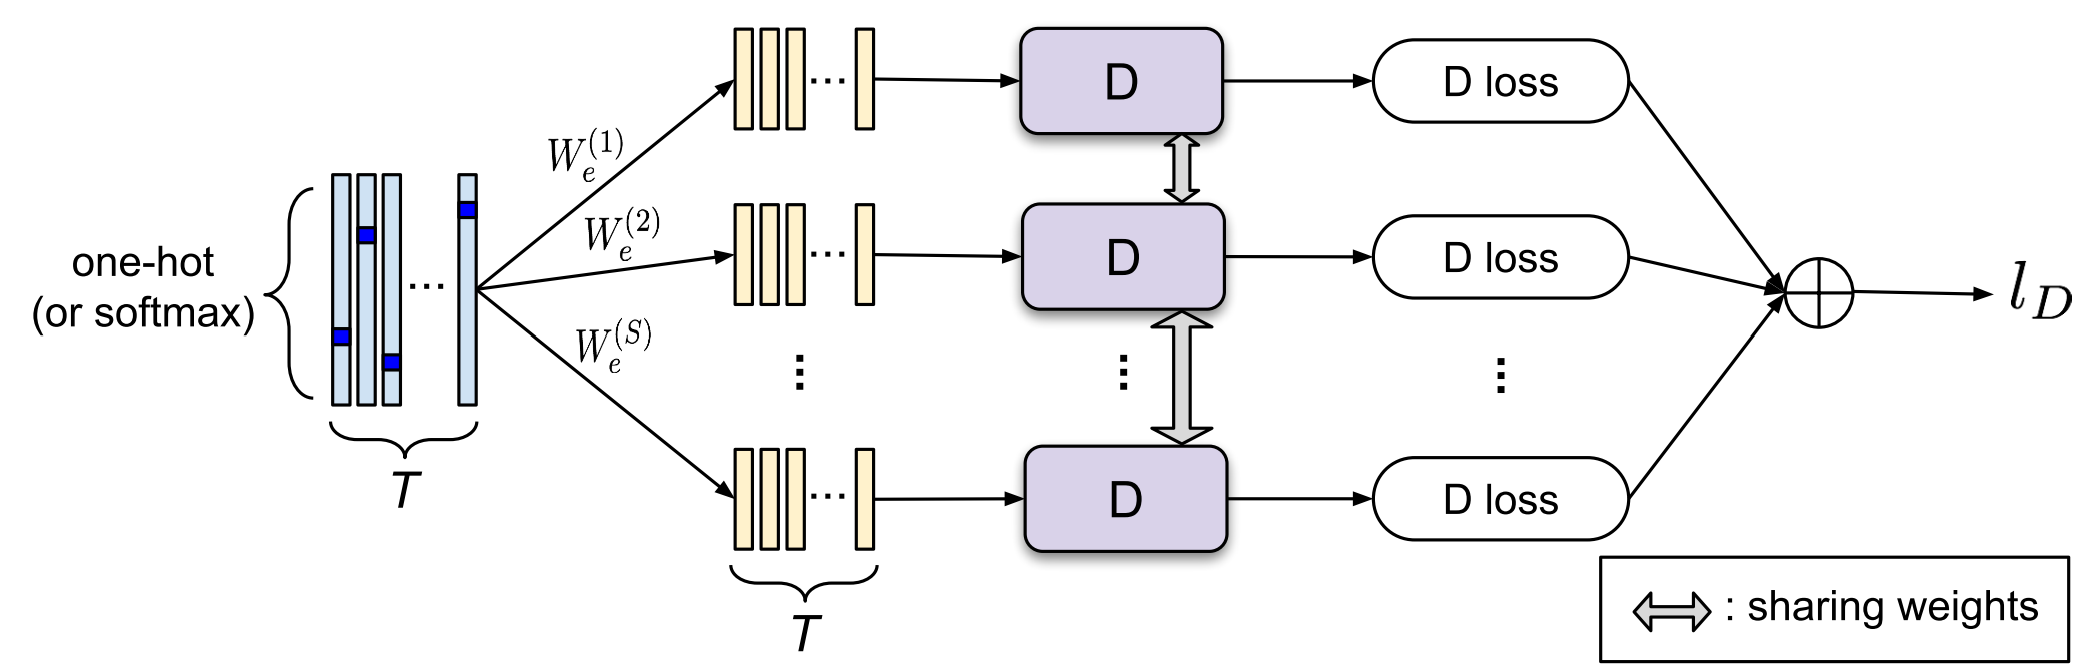
\includegraphics[width=0.8\linewidth]{Images/MultipleDiscriminator.png}
		\caption{Multiple Discriminator}
		\label{img:MultipleDiscriminator}
	\end{figure}
\end{enumerate}

\textbf{
Lot of this work can be based on a Survey done 1-2 years ago \cite{Lu} \\
There there are many other works that speaks about GAN and what I want to point out is that all these works are really new. New in the sense of the last months. \\
This is what I would like to show that everything is based on something really new. \cite{Chen} \cite{DeMasson} \cite{Dieng} \cite{Fedus2018} \cite{RelGAN} \cite{Guo} \cite{Lin2018} \cite{Wang2018} \cite{Yu2016} \cite{Zhang2017} \\
This is not a GAN based model but it is done using Variational Autoencoders \cite{Wang}
}
\subsection{Transformer Based}
Here there could be a big section related to all the works based on language models trained on big corpus like Bert and recent works on GPT by OpenAI
